\chapter{Технологический раздел}

В этом разделе выбраны средства реализации, описана программная реализация модуля модификации поведения на основе персональных черт, проведено тестирование.

\section{Выбор средств реализации}

Для реализации метода выбран язык программирования Python~\cite{info_pl} по следующим причинам:

\begin{itemize}
	\item в рамках дисциплины <<Программирование>>, <<Планирование эксперимента>> и др. данный язык был подробно изучен и многократно применялся при решении задач;
	\item в данном языке есть библиотека Simpful, предоставляющая необходимые функции для реализации нечётких множеств и нечёткого вывода~\cite{spolaor2020simpful}.
\end{itemize}

В качестве среды разработки был выбран PyCharm~\cite{pycharm_ide} по следующим причинам:

\begin{itemize}
	\item данная среда разработки создана специально для написания приложения на языке Python~\cite{pycharm_ide};
	\item в данной среде разработки имеется множество расширений для работы с утилитой make~\cite{stallman2006gnuMake}, bash-скриптами~\cite{bash_scripts_docs}.
\end{itemize}

Для тестирования выбрана стандартная библиотека \texttt{unittest}~\cite{python_unittest_docs}.

\section{Сведения о модулях программы}

Программное обеспечение состоит из следующих модулей:

\begin{itemize}
	\item \texttt{f2robot\_client.py} --- формирование HTTP-запроса на сервер робота Ф-2, отправка сообщения пользователя, извлечение пар
	\texttt{scenario}/\texttt{proximity} из JSON-тела ответа;
	\item \texttt{f2robot\_personality\_filter.py} --- реализация модуля модификации поведения на основе персональных черт --- описание термов, правил, фаззификации и перевзвешивания д-сценариев;
	\item \texttt{f2robot\_profile\_config.py} --- загрузка JSON-конфигураций профилей
	робота, параметров отношений и ситуаций, правил для
	модуля модификации поведения;
	\item \texttt{GUI.py} --- графический интерфейс пользователя;
	\item \texttt{main.py} --- точка входа в программу.
\end{itemize}

\section{Конфигурация профиля (характера) робота}

Конфигурация профиля (характера) робота задаётся набором JSON-файлов.
Названия и назначения файлов приведены в таблице~\ref{tbl:json_config_files}.

\begin{table}[H]
	\centering
	\caption{Назначение JSON-файлов конфигурации}
	\label{tbl:json_config_files}
	\begin{tabularx}{\textwidth}{|p{0.34\textwidth}|X|}
		\hline
		\textbf{Файл} & \textbf{Назначение} \\
		\hline
		\texttt{trait\_profile.json} & Список значений персональных черт робота \\
		\hline
		\texttt{relation\_params.json} & Список параметров отношения робота к собеседнику, например, круг общения \\
		\hline
		\texttt{situation\_params.json} & Список параметров ситуации \\
		\hline
		\texttt{rules.json} & Список правил перевзвешивания д-сценариев:
		условия, целевые сценарии и эффект. \\
		\hline
	\end{tabularx}
\end{table}

На рисунке~\ref{img:profile} приведен пример содержимого файла \texttt{trait\_profile.json} с набором черт и выбранными для них термами.

\includeimage
{profile}
{f}
{H}
{0.6\textwidth}
{Пример содержимого файла \texttt{trait\_profile.json}}


Назначение полей в файле \texttt{trait\_profile.json}:
\begin{itemize}
	\item \texttt{section} --- тип конфигурационного файла для проверки
	корректности загружаемого раздела;
	\item \texttt{profile\_id} --- идентификатор профиля робота;
	\item \texttt{label} --- отображаемое в интерфейсе название профиля;
	\item \texttt{traits} --- значения персональных черт робота;
	\item \texttt{value} --- выбранный терм черты;
	\item \texttt{label} --- отображаемое в интерфейсе название терма.
\end{itemize}

Параметры отношения робота к собеседнику и параметры ситуации описываются как элементы массива \texttt{parameters}.
Для дискретных параметров используется поле \texttt{options}.
На рисунке~\ref{img:relation} приведен пример описанного параметра отношения робота к собеседнику:

\includeimage
{relation}
{f}
{H}
{0.5\textwidth}
{Пример описанного дискретного параметра}

Назначение полей в файлах \texttt{situation\_params.json} и \texttt{relation\_params.json} для дискретных параметров:
\begin{itemize}
	\item \texttt{section} --- тип файла с параметрами отношения к собеседнику;
	\item \texttt{parameters} --- список настраиваемых параметров;
	\item \texttt{feature} --- имя параметра;
	\item \texttt{label} --- отображаемое в интерфейсе название параметра;
	\item \texttt{input} --- тип элемента интерфейса для ввода значения ---
	\texttt{select} для выбора из списка или \texttt{slider} для ввода
	численного значения на шкале;
	\item \texttt{default} --- значение параметра по умолчанию;
	\item \texttt{options} --- допустимые дискретные значения;
	\item \texttt{term} --- имя значения;
	\item \texttt{label} --- отображаемое в интерфейсе название значения.
\end{itemize}

Для численных параметров используются границы шкалы и термы нечёткой переменной.
Пример приведён на рисунке~\ref{img:situation}.

\includeimage
{situation}
{f}
{H}
{0.6\textwidth}
{Пример описанного численного параметра}

Назначение полей в файлах \texttt{situation\_params.json} и \texttt{relation\_params.json} для численных параметров:
\begin{itemize}
	\item \texttt{feature} --- имя численного параметра ситуации;
	\item \texttt{label} --- отображаемое в интерфейсе название параметра;
	\item \texttt{input} --- тип элемента интерфейса для ввода значения ---
	\texttt{select} для выбора из списка или \texttt{slider} для ввода
	численного значения на шкале;
	\item \texttt{default} --- численное значение по умолчанию;
	\item \texttt{minimum} и \texttt{maximum} --- диапазон значений параметра;
	\item \texttt{fuzzy\_terms} --- термы нечёткой переменной;
	\item \texttt{term} --- имя терма;
	\item \texttt{label} --- отображаемое в интерфейсе название терма;
	\item \texttt{function\_type} --- тип функции принадлежности ---
	\texttt{triangle} для треугольной функции по трём точкам или
	\texttt{trapezoid} для трапециевидной функции по четырём точкам;
	\item \texttt{points} --- опорные точки функции принадлежности.
\end{itemize}

Правило связывает условия с одним или несколькими д-сценариями и эффектом.
Пример правила приведен на рисунке~\ref{img:rules}.

\includeimage
{rules}
{f}
{H}
{0.7\textwidth}
{Пример описанного правила в файле\texttt{rules.json}}

Назначение полей в файле \texttt{rules.json}:
\begin{itemize}
	\item \texttt{rule\_id} --- уникальный идентификатор правила;
	\item \texttt{label} --- отображаемое в интерфейсе описание правила;
	\item \texttt{conditions} --- условия срабатывания правила;
	\item \texttt{feature} --- проверяемый признак;
	\item \texttt{terms} --- допустимые термы признака;
	\item \texttt{target\_scenarios} --- д-сценарии, вес которых изменяется при
	срабатывании правила;
	\item \texttt{effect} --- значение изменения веса сценария.
\end{itemize}

Загрузка перечисленных JSON-файлов выполняется модулем
\texttt{f2robot\_profile\_config.py}.

\section{Реализация клиента Ф-2}

Модуль \texttt{f2robot\_client.py} выполняет три основные функции:

\begin{enumerate}
	\item формирует тело HTTP-запроса к серверу робота Ф-2;
	\item отправляет POST HTTP-запрос к серверу робота Ф-2;
	\item выполняет выборку полей из JSON-ответа, приводит ответ к компактному набору пар
	\texttt{scenario}/\texttt{proximity}.
\end{enumerate}

При отправке запроса задаётся тайм-аут 30 секунд, по истечении тайм-аута пользователю выводится сообщение об ошибке.

\section{Реализация модуля модификации поведения на основе персональных черт}

Центральным модулем является \texttt{f2robot\_personality\_filter.py}.
В нём описаны структуры данных и функции, необходимые для применения правил.

Для описания предметных сущностей используются классы данных:

\begin{itemize}
	\item \texttt{Condition} задаёт одно условие правила --- имя признака и набор
	допустимых термов;
	\item \texttt{FilterRule} задаёт правило перевзвешивания д-сценариев;
	\item \texttt{RuleActivation} хранит факт срабатывания правила;
	\item \texttt{FilteredScenario} хранит исходный и модифицированный вес
	д-сценария;
	\item \texttt{FuzzyTermSpec} описывает терм и параметры функции
	принадлежности;
	\item \texttt{FuzzyVariableSpec} описывает нечёткую переменную.
\end{itemize}

Численные признаки профиля, отношения и ситуации фаззифицируются при выполнении
правил классом \texttt{SimpfulRuleEngine}.
Для каждой нечёткой переменной задаётся область значений и набор термов.
Могут применяться треугольные и трапециевидные функции принадлежности.

Например, для признака \texttt{offensiveness\_degree} используются термы
\texttt{low}, \texttt{medium}, \texttt{high}.
При значении \texttt{offensiveness\_degree = 0.60} признак частично принадлежит сразу двум соседним термам: \texttt{medium} и \texttt{high}.
Это позволяет правилу сработать не только полностью или совсем не сработать, но и с промежуточной силой.

\section{Интерфейс программы}

Графический интерфейс изображен на рисунках~\ref{img:gui_setup} и~\ref{img:gui_result} и содержит две основные вкладки: \texttt{Настройка} и \texttt{Результат}.
В верхней части окна отображается количество загруженных правил и нечётких
признаков текущего профиля.

\begin{figure}[H]
	\centering
	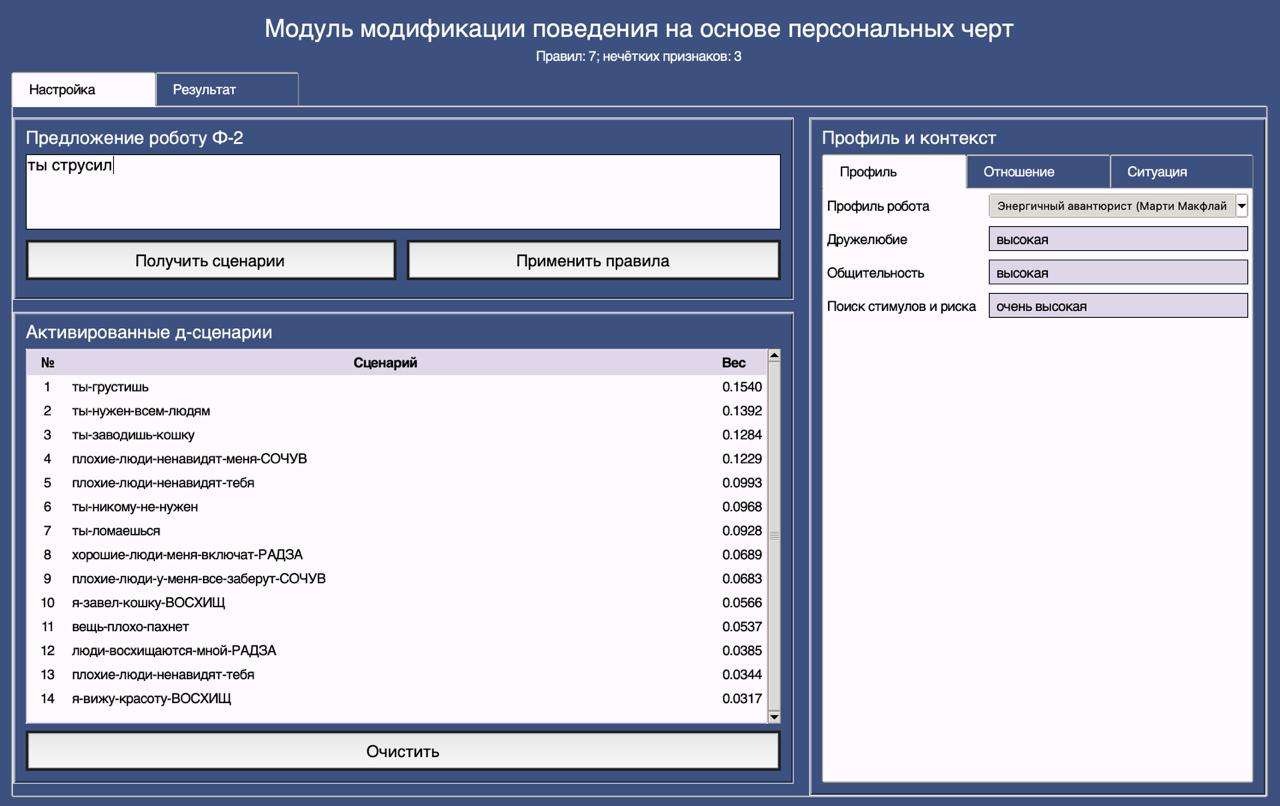
\includegraphics[width=1\textwidth]{inc/img/gui_setup.png}
	\caption{Вкладка настройки профиля, контекста и активированных д-сценариев}
	\label{img:gui_setup}
\end{figure}

Вкладка \texttt{Настройка} используется для ввода предложения, получения
активированных д-сценариев и задания контекста работы модуля.

Блок \texttt{Предложение роботу Ф-2} содержит следующие элементы:
\begin{itemize}
	\item поле ввода предложения пользователя --- текст, который отправляется на сервер Ф-2;
	\item кнопка \texttt{Получить сценарии} --- отправка предложения на сервер Ф-2 и
	заполнение списка активированных д-сценариев;
	\item кнопка \texttt{Применить правила} --- запуск локального
	перевзвешивания д-сценариев по выбранному профилю и параметрам контекста.
\end{itemize}

Блок \texttt{Активированные д-сценарии} содержит следующие элементы:
\begin{itemize}
	\item столбец \texttt{Сценарий} --- имя д-сценария, полученного от Ф-2;
	\item столбец \texttt{Вес} --- исходный вес д-сценария;
	\item кнопка \texttt{Очистить} --- удаление всех д-сценариев из списка.
\end{itemize}

Блок \texttt{Профиль и контекст} содержит вкладки параметров:
\begin{itemize}
	\item вкладка \texttt{Профиль} --- выбор профиля робота и отображение
	значений его персональных черт;
	\item вкладка \texttt{Отношение} --- настройка параметров отношения к
	собеседнику;
	\item вкладка \texttt{Ситуация} --- настройка параметров текущей ситуации.
\end{itemize}

\begin{figure}[H]
	\centering
	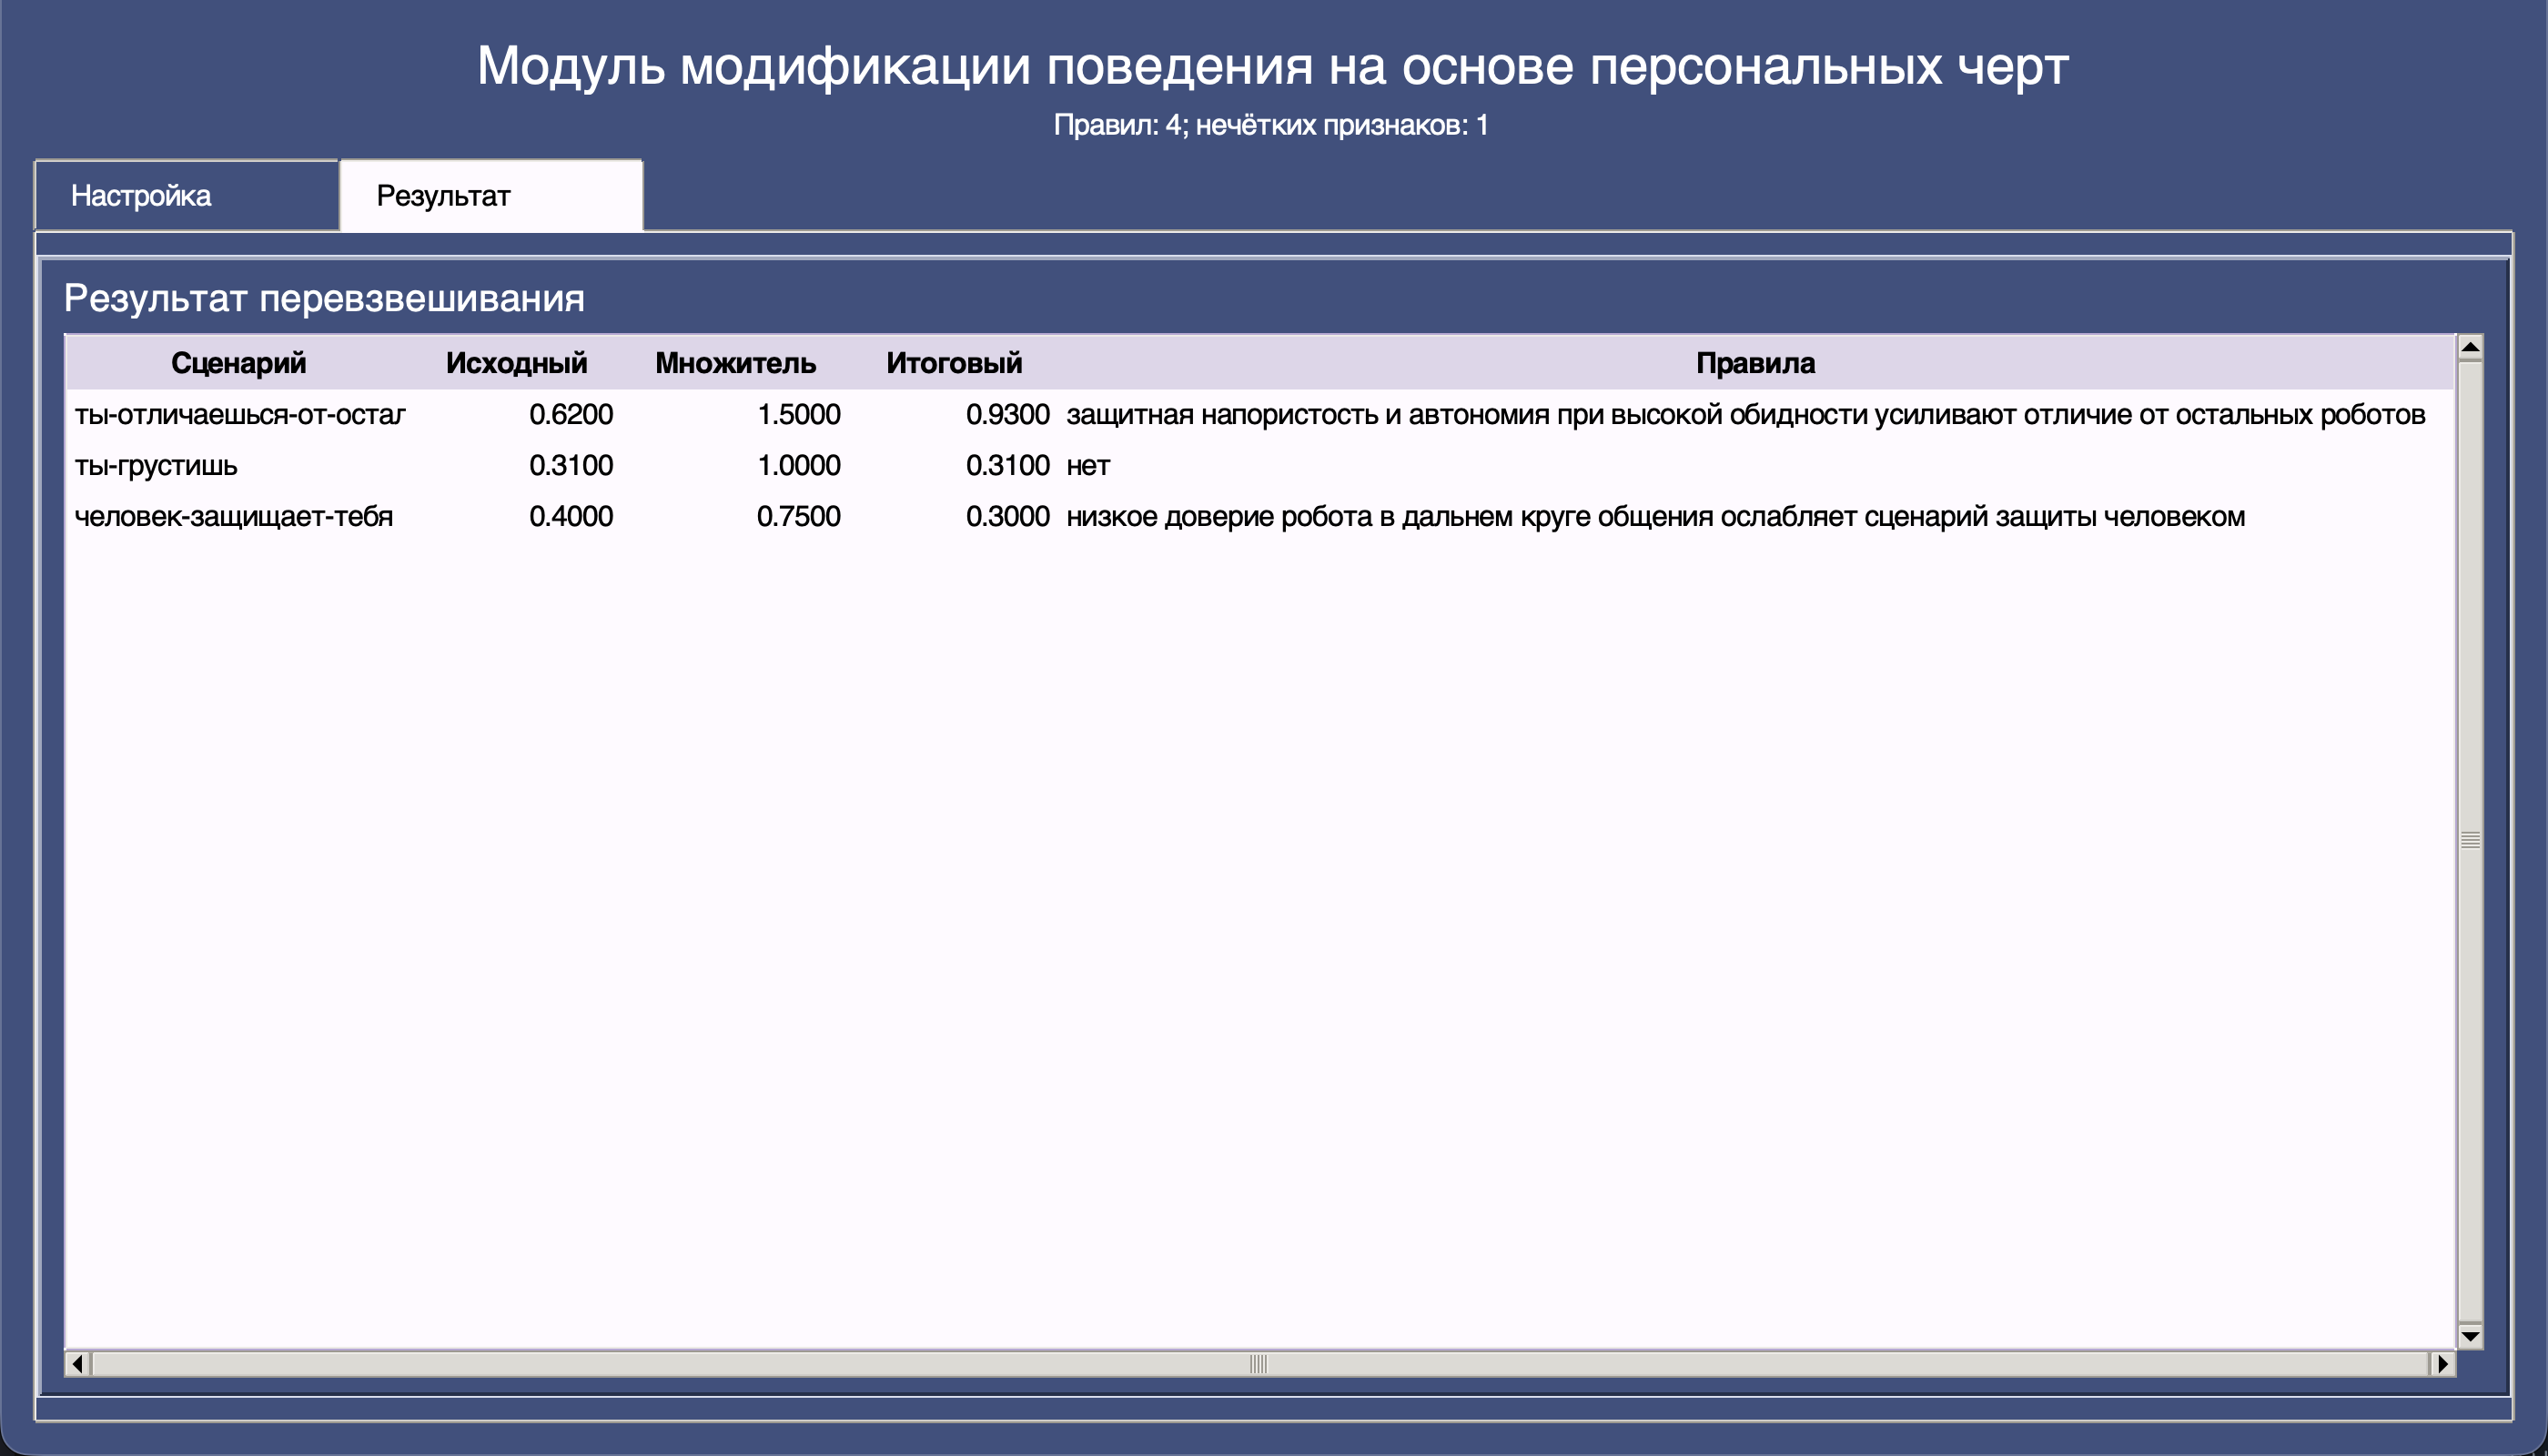
\includegraphics[width=1\textwidth]{inc/img/gui_result.png}
	\caption{Вкладка результата перевзвешивания д-сценариев}
	\label{img:gui_result}
\end{figure}

Вкладка \texttt{Результат} показывает итог работы модуля.
Блок \texttt{Результат перевзвешивания} содержит таблицу со следующими
столбцами:
\begin{itemize}
	\item \texttt{Сценарий} --- имя обработанного д-сценария;
	\item \texttt{Исходный} --- вес д-сценария до применения правил;
	\item \texttt{Множитель} --- итоговый множитель, рассчитанный по
	сработавшим правилам;
	\item \texttt{Итоговый} --- вес д-сценария после перевзвешивания;
	\item \texttt{Правила} --- правила, которые повлияли на расчёт, или
	значение \texttt{нет}, если правила не сработали.
\end{itemize}


\section{Функциональное тестирование}

\subsection*{Позитивные тесты}

Результаты позитивных тестов приведены в
таблице~\ref{tbl:functional_test_results}.

\begin{longtable}{|p{0.11\textwidth}|p{0.27\textwidth}|p{0.35\textwidth}|p{0.16\textwidth}|}
	\caption{Результаты позитивных тестов}
	\label{tbl:functional_test_results} \\
	\hline
	\textbf{Номер теста} & \textbf{Проверяемый случай} & \textbf{Ожидаемое поведение} & \textbf{Результат} \\
	\hline
	\endfirsthead
	\caption[]{Результаты позитивных тестов (продолжение)} \\
	\hline
	\textbf{Номер теста} & \textbf{Проверяемый случай} & \textbf{Ожидаемое поведение} & \textbf{Результат} \\
	\hline
	\endhead
	\hline
	\endfoot
	\endlastfoot
	1 & Передано одно предложение для отправки на сервер робота Ф-2 &
	Сформированное тело запроса содержит массив \texttt{variants} с
	единственным элементом, равным исходному предложению & Тест пройден \\
	\hline
	2 & В файле \texttt{.env} задан адрес сервера робота Ф-2 & Клиент считывает
	значение требуемой переменной и возвращает адрес &
	Тест пройден \\
	\hline
	3 & В файле окружения присутствуют адрес сервера робота Ф-2 и посторонняя
	переменная & Клиент использует значение только переменной, имя которой
	задано в его конфигурации & Тест пройден \\
	\hline
	4 & Адрес сервера робота Ф-2 задан и в переменной окружения, и в файле
	\texttt{.env} & Клиент использует значение из файла \texttt{.env},
	заменяя им ранее установленное значение переменной окружения &
	Тест пройден \\
	\hline
	5 & Робот Ф-2 вернул набор сценариев, среди которых присутствуют сценарии,
	начинающиеся с символа \texttt{@} & Клиент робота отсеивает сценарии,
	начинающиеся с символа \texttt{@}, формируя итоговое множество
	сценариев. & Тест пройден \\
	\hline
	6 & Загружаются JSON-файлы выбранного тестового
	профиля & Успешная загрузка всех 4-х файлов профиля. & Тест пройден \\
	\hline
	7 & В каталоге профилей находятся два каталога с корректными
	файлами \texttt{trait\_profile.json} & Оба профиля обнаруживаются в
	порядке имён каталогов; их идентификаторы, подписи и пути соответствуют
	JSON-файлам & Тест пройден \\
	\hline
	8 & Загружаются профили без явного указания загружаемого профиля & По умолчанию загружается первый профиль из упорядоченного
	списка доступных профилей & Тест пройден \\
	\hline
	9 & Загружаются профили с явным указанием загружаемого профиля & Загружаются только указанный профиль & Тест пройден. \\
	\hline
	10 & Загружается профиль, правила которого покрывают
	все настроенные термы и используют определённые эффекты & Успешная загрузка профиля & Тест пройден \\
	\hline
	11 & Загружается профиль, содержащий все обязательные
	подписи & Успешная загрузка профиля & Тест пройден \\
	\hline
	12 & В модуль переданы численные признаки ситуации & Для каждого
	признака вычисляются ожидаемые степени принадлежности термам в
	соответствии с заданными функциями принадлежности & Тест пройден \\
	\hline
	13 & Численный параметр отношения к собеседнику используется в
	условии правила & Параметр фаззифицируется; рассчитанная степень
	принадлежности определяет активацию правила, множитель и итоговый вес
	д-сценария & Тест пройден \\
	\hline
	14 & Для одного д-сценария одновременно срабатывают два правила. &
	Итоговый множитель д-сценария рассчитывается как взвешенное среднее
	множителей сработавших правил & Тест пройден \\
	\hline
	15 & Входной д-сценарий содержит вес в поле \texttt{proximity} &
	Значение \texttt{proximity} используется как исходный вес
	д-сценария при перевзвешивании & Тест пройден. \\
	\hline
\end{longtable}

Все тесты были пройдены успешно.

\subsection*{Негативные тесты}

Результаты негативных тестов приведены в таблице~\ref{tbl:negative_functional_test_results}.

\begin{longtable}{|p{0.11\textwidth}|p{0.27\textwidth}|p{0.35\textwidth}|p{0.16\textwidth}|}
	\caption{Результаты негативных тестов}
	\label{tbl:negative_functional_test_results} \\
	\hline
	\textbf{Номер теста} & \textbf{Проверяемый случай} & \textbf{Ожидаемое поведение} & \textbf{Результат} \\
	\hline
	\endfirsthead
	\caption[]{Результаты негативных тестов (продолжение)} \\
	\hline
	\textbf{Номер теста} & \textbf{Проверяемый случай} & \textbf{Ожидаемое поведение} & \textbf{Результат} \\
	\hline
	\endhead
	\hline
	\endfoot
	\endlastfoot
	1 & Для отправки на сервер робота Ф-2 передано пустое предложение &
	Формирование тела запроса завершается исключением \texttt{ValueError} &
	Тест пройден. \\
	\hline
	2 & Клиент создаётся при отсутствии адреса сервера робота Ф-2 в окружении &
	Создание клиента завершается исключением \texttt{RuntimeError}, текст
	которого содержит имя требуемой переменной & Тест пройден \\
	\hline
	3 & JSON-ответ Ф-2 содержит только сценарии, имена которых начинаются
	с символа \texttt{@} & Клиент возвращает пустой список
	\texttt{scenario\_proximities} & Тест пройден \\
	\hline
	4 & В фильтр передаётся правило без условий & Создание фильтра
	завершается исключением \texttt{ValueError} & Тест пройден. \\
	\hline
	5 & В каталоге профиля отсутствует один из 4-х файлов профиля &
	Загрузка профиля завершается исключением
	\texttt{FileNotFoundError}, содержащим имя отсутствующего файла &
	Тест пройден. \\
	\hline
	6 & В каталоге профилей отсутствуют профили &
	Загрузка профилей завершается исключением \texttt{RuntimeError},
	сообщающим об отсутствии доступных профилей & Тест пройден. \\
	\hline
	7 & Один из настроенных термов не используется ни в одном условии
	правил профиля & При загрузке профиля выводится предупреждение \texttt{UserWarning}, содержащее
	непокрытый терм & Тест пройден \\
	\hline
	8 & Для используемого эффекта правила отсутствует подпись &
	Загрузка профиля завершается исключением \texttt{ValueError},
	содержащим имя эффекта без подписи & Тест пройден \\
	\hline
	9 & В одном из JSON-файлов профиля отсутствует обязательный
	верхнеуровневый ключ & Загрузка профиля завершается исключением
	\texttt{ValueError}, содержащим имя отсутствующего ключа &
	Тест пройден. \\
	\hline
\end{longtable}

Все тесты пройдены успешно.

\phantomsection
\section*{Выводы}
\addcontentsline{toc}{section}{Выводы}

В технологическом разделе выбраны средства реализации программного
обеспечения и приведена его модульная структура.
Описана конфигурация профиля робота, параметров отношения,
параметров ситуации, правил и эффектов перевзвешивания.
Также рассмотрены реализация клиента сервера Ф-2, модуля модификации поведения на
основе персональных черт и графического интерфейса программы.
Было проведено функциональное тестирование.
